% Mid-submission progress report. Numbers come from pretrained/scripts/make_tables.py
% (results/tables/*.md) and per-run summaries; decisions referenced as D-xx are in Plan/Decision_Log.md.
%   cd pretrained && .venv/bin/python scripts/make_tables.py && cd ../Reports/Mid && latexmk -pdf PreTrained_Mid.tex
\documentclass[11pt,a4paper]{article}

\usepackage[margin=2.2cm]{geometry}
\usepackage[T1]{fontenc}
\usepackage{lmodern}
\usepackage{microtype}
\usepackage{amsmath}
\usepackage{xcolor}
\usepackage{booktabs}
\usepackage{tabularx}
\usepackage{array}
\usepackage{enumitem}
\usepackage{caption}
\usepackage{float}
\usepackage{titlesec}
\usepackage{tikz}
\usetikzlibrary{arrows.meta,positioning,fit,backgrounds,calc}
\usepackage[hidelinks]{hyperref}

\definecolor{accent}{HTML}{0E6B5C}
\definecolor{soft}{HTML}{E4F1EE}
\definecolor{warn}{HTML}{B4492C}
\definecolor{muted}{HTML}{56635E}

\titleformat{\section}{\large\bfseries\color{accent}}{\thesection}{0.6em}{}
\titleformat{\subsection}{\normalsize\bfseries}{\thesubsection}{0.5em}{}
\titlespacing*{\section}{0pt}{1.1em}{0.4em}
\titlespacing*{\subsection}{0pt}{0.8em}{0.3em}
\setlist{itemsep=1pt,topsep=3pt,leftmargin=1.4em}
\captionsetup{font=small,labelfont=bf}
\newcolumntype{L}{>{\raggedright\arraybackslash}X}
\newcolumntype{P}[1]{>{\raggedright\arraybackslash\hyphenpenalty=10000}p{#1}}
\renewcommand{\arraystretch}{1.15}
\setlength{\emergencystretch}{3em}

\newcommand{\up}[1]{\textbf{\color{accent}#1}}
\newcommand{\down}[1]{\textbf{\color{warn}#1}}

\begin{document}

\begin{center}
  {\LARGE\bfseries Requirements as the Oracle}\\[3pt]
  {\large Generating REST API Tests from Vague Requirements Without Learning the Bugs They Should Catch}\\[6pt]
  {\large Mid-term progress report}\\[8pt]
  {\large\bfseries Team PreTrained}\\[4pt]
  {\small\begin{tabular}{@{}l@{\hspace{1.2em}}l@{\hspace{3em}}l@{\hspace{1.2em}}l@{}}
Sohail Memon & 2025201075 & Mohd Ahmad & 2025201029\\
Kathan Patel & 2025201039 & Md Taufique Hussain & 2025202007
\end{tabular}}\\[6pt]
  {\small Code: \url{https://github.com/SohailTSM/Requirements-as-the-Oracle}}
\end{center}

%-------------------------------------------------------------------- 1
\section{Summary of progress}
We are building an LLM agent that writes REST API tests from \emph{vague} natural-language requirements plus an OpenAPI specification, using only Llama~3.1~8B. Two questions drive the work. First, can a small model catch requirement bugs from vague wording? Second, can refinement against a possibly buggy service be made safe, so that the test does not learn the bug it should catch? We evaluate on RESTestBench~\cite{restestbench}.

\begin{itemize}
\item \textbf{Built.} The full pipeline runs end to end through RESTestBench's unmodified harness. It comprises retrieval, the precision layer, the planner, lint and specification clean-up, the compiler, execution, the judge and guarded refinement. All 27 component variants of the proposal are implemented, including ReAct, multi-persona, blackboard, MCP and A2A, as are baselines B1--B4 and the fuzzer.
\item \textbf{Run.} 69 of the 81 planned baseline runs (one run = one service) are complete: every NestJS and TodoApp baseline, the fuzzer, B1 and half of B2/B3 on FastAPI. 24 of the 27 sweep rows are done, with the default configuration repeated 3 times; the remaining 3 rows need the fine-tuned models. Retrieval and the precision layer are evaluated offline. SFT fine-tuning (3 leave-one-service-out folds) is trained, merged and installed.
\item \textbf{Main result so far.} Refining against the buggy service halves the score of RESTestBench's refinement loop (B2) on FastAPI: 17.0\% of planted bugs caught when it refines against the correct service, 8.1\% against the buggy one. Our pipeline loses almost nothing (12.0\% vs 11.3\% for the default; about 17\% in both settings for the best variants). So on the realistic setting, where the service may be buggy, our best variants catch about twice as many bugs as B2 (Section~\ref{sec:adapt}).
\item \textbf{Main weakness.} About 70\% of our tests still fail on the \emph{correct} service, mostly because the precision layer derives checks that contradict the real requirement.
\end{itemize}
Every design decision and its reason is logged (\texttt{Plan/Decision\_Log.md}, D-01 to D-112).

%-------------------------------------------------------------------- 2
\section{System}
\begin{figure}[H]\centering
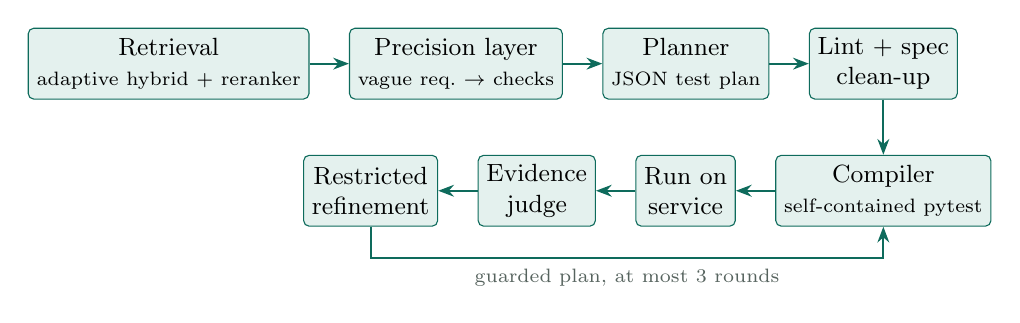
\begin{tikzpicture}[node distance=4mm and 5mm, box/.style={draw=accent, fill=soft, rounded corners=2pt, align=center, font=\small, minimum height=9mm, inner sep=3pt}, arr/.style={-{Stealth[length=2mm]}, accent, thick}]
\node[box] (ret) {Retrieval\\\scriptsize adaptive hybrid + reranker};
\node[box, right=of ret] (pre) {Precision layer\\\scriptsize vague req.\ $\to$ checks};
\node[box, right=of pre] (plan) {Planner\\\scriptsize JSON test plan};
\node[box, right=of plan] (lint) {Lint + spec\\clean-up};
\node[box, below=7mm of lint] (comp) {Compiler\\\scriptsize self-contained pytest};
\node[box, left=of comp] (run) {Run on\\service};
\node[box, left=of run] (judge) {Evidence\\judge};
\node[box, left=of judge] (ref) {Restricted\\refinement};
\draw[arr] (ret) -- (pre); \draw[arr] (pre) -- (plan); \draw[arr] (plan) -- (lint); \draw[arr] (lint) -- (comp);
\draw[arr] (comp) -- (run); \draw[arr] (run) -- (judge); \draw[arr] (judge) -- (ref);
\draw[arr] (ref.south) -- ++(0,-4mm) -| node[pos=0.25, below, font=\scriptsize, muted]{guarded plan, at most 3 rounds} (comp.south);
\end{tikzpicture}
\caption{Default pipeline. Everything before the run step uses only the requirement and the specification frozen from the correct service.}
\end{figure}

\textbf{The model writes a plan, not code.} The LLM writes a structured plan (actors, calls, checks). A deterministic compiler turns the plan into a self-contained pytest file. The plan can then be checked against the specification before any call, and refinement knows exactly which expected values are locked.

\textbf{Safety rules for refinement.}
\begin{enumerate}[label=(\arabic*)]
\item On assertion failures, refinement sees status codes and field names but never response values.
\item A strengthen-only guard restores any change to a meaning check, and blocks new expected values copied from a response.
\item Field repairs must land on fields the specification documents.
\item The judge may blame the test only with evidence from the requirement or the specification.
\end{enumerate}
\textbf{Specification-only clean-up.} Before execution, plan errors are fixed deterministically, e.g.\ missing path parameters are filled in and checks the specification shows can never pass are dropped.

%-------------------------------------------------------------------- 3
\section{Datasets}
\begin{table}[H]\centering\small
\begin{tabularx}{\linewidth}{@{}P{3.3cm}L@{}}
\toprule
\textbf{Dataset} & \textbf{Content and use}\\\midrule
RESTestBench~\cite{restestbench} (public) & 3 Dockerised services: FastAPI (Python), NestJS RealWorld (TypeScript), TodoApp (.NET). 106 requirements (63 / 29 / 14), each in a vague and a precise version; 228 hand-written planted bugs (mutants; 141 / 65 / 22); one reference test per requirement; scoring harness. The agent sees only the vague text and the specification. Precise text is used only for scoring and gold data.\\
Gold operations (ours) & For each requirement, the specification operations its reference test uses (106 requirements). Ground truth for retrieval.\\
Gold checks (ours) & 268 atomic checks drafted by Claude from the precise requirements. Ground truth for the precision layer. Being validated by human labels (below).\\
Reference plans (ours) & 10 hand-written plans for FastAPI that pass the correct service 10/10 and catch 26 of 28 planted bugs. Used to check that the compiler and runtime are correct.\\
SFT data (ours) & Vague requirement $\to$ verified checks, one fold per held-out service; 86--184 examples per fold.\\
DPO data (ours) & ``Report the bug'' (chosen) vs ``copy the observed value'' (rejected) refinement pairs. Built from guarded runs; collection still pending.\\
Human-validation set & 45 requirements, 181 labels (are the gold checks correct, and do the precision layer's checks cover them), on a shared labelling page. Gives Cohen's $\kappa$ between labellers and against the Llama judge.\\
\bottomrule
\end{tabularx}
\caption{Datasets used.}
\end{table}

%-------------------------------------------------------------------- 4
\section{Experimental setup}
\textbf{Model and compute.} Every LLM role uses Llama~3.1~8B Instruct, 4-bit (Q4\_K\_M) under Ollama, with 24k context, temperature 0.2 and at most 3 refinement rounds. The baselines are rerun on the same model, so every comparison is like for like.
\begin{itemize}
\item Early runs used the team's RTX~5050 laptop. Most runs since 23 Oct use Kaggle T4 servers on the four team accounts, reached through a tunnel. A local request dispatcher sends each LLM call to the next free slot (2 requests per T4 measured at $1.40\times$ throughput).
\item The services under test run locally in Docker, with up to 10 FastAPI copies at once so that scoring never leaves a model slot idle.
\item The harness is pinned and never edited.
\item FastAPI is the development service; NestJS and TodoApp are held out from every design decision.
\end{itemize}

\textbf{Metrics.}
\begin{itemize}
\item \emph{Caught}: percentage of planted bugs caught by tests generated while interacting with the correct service. A test counts only if it passes on the correct service. This is RESTestBench's score.
\item \emph{Mutant-gen}: the same score for tests generated while interacting with the buggy service, which is the realistic setting.
\item \emph{Adaptation gap}: Caught minus Mutant-gen.
\item \emph{Pass-OK}: share of tests that pass on the correct service.
\item Component metrics: retrieval Recall@5, ``all needed operations in the top 5'' and MRR; precision-layer recall, contradiction and unsupported rates against the gold checks.
\end{itemize}

%-------------------------------------------------------------------- 5
\section{Baseline experiments}
\begin{enumerate}[label=\textbf{B\arabic*}]
\item Single-step generation, RESTestBench's own tool.
\item RESTestBench's refinement loop, unchanged.
\item B2 with only the prompts fixed: the copying example removed, the generator warned, judge feedback passed on, and an \textsc{API\_BUG} outcome added.
\item A response-judging agent in the style of LogiAgent~\cite{logiagent}.
\end{enumerate}
\textbf{E} is the Schemathesis fuzzer. It uses a crash/schema oracle and no requirements.

\begin{table}[H]\centering\small
\begin{tabular}{llrrrc}\toprule
Tool & Wording & FastAPI & NestJS & TodoApp & Runs (FastAPI / others)\\\midrule
B1 single-step & precise & 39.7 $\pm$ 2.6 & 5.1 $\pm$ 1.8 & 1.5 $\pm$ 2.6 & 3 / 3\\
B2 refinement & precise & 49.6 & 6.2 $\pm$ 2.7 & 0.0 & 1 / 3\\
B3 prompt-fixed & precise & 36.2 & 5.6 $\pm$ 4.9 & 0.0 & 1 / 3\\
B4 response judge & precise & \emph{queued} & 10.3 $\pm$ 5.8 & 4.5 & 0 / 3\\\midrule
B1 single-step & vague & 4.3 $\pm$ 1.4 & 0.0 & 0.0 & 3 / 3\\
B2 refinement & vague & 17.0 $\pm$ 3.0 & 0.0 & 4.5 & 2 / 3\\
B3 prompt-fixed & vague & 4.3 $\pm$ 4.0 & 0.0 & 0.0 & 2 / 3\\
B4 response judge & vague & \emph{queued} & 3.1 $\pm$ 4.1 & 18.2 & 0 / 3\\\midrule
E fuzzer & -- & 13.9 $\pm$ 7.8 & 0.0 & 9.1 & 3 / 3\\
\bottomrule\end{tabular}
\caption{Baselines: planted bugs caught (\%), mean $\pm$ sd over complete runs. Runs still in progress are left out. The remaining FastAPI runs are queued.}
\label{tab:baselines}
\end{table}
\textbf{Observations.}
\begin{itemize}
\item \textbf{Vague wording collapses single-step generation.} On FastAPI, B1 catches 40\% of planted bugs from precise requirements but 4\% from vague ones, and 95\% of its vague tests fail even on the correct service. This is the gap our method targets.
\item \textbf{Fixing the prompts alone does not help on vague wording.} B3 scores 4.3\% against B2's 17.0\%. B3's judge answered \textsc{API\_BUG} in 36 of 36 TodoApp rounds, so it almost never refines: the 8B model takes the ``it's the API's fault'' option whenever it is offered.
\item \textbf{NestJS and TodoApp are near zero for every LLM baseline.} On TodoApp the model registers users with weak passwords that the service's undocumented password policy rejects; our runtime generates strong credentials for actors. These services are held out and will show whether our pipeline generalises.
\item \textbf{B2 copies response values.} In 12--22\% of its refinement rounds, B2 adds an asserted literal taken from the previous HTTP response. This is exactly the behaviour our guard blocks.
\end{itemize}

%-------------------------------------------------------------------- 6
\section{Our agent: component sweep (one-at-a-time ablations)}
Starting from the default configuration, the sweep changes one component at a time on all 63 FastAPI requirements (vague wording, 1 run each). Removal rows (no precision layer, no refinement, no judge, full specification instead of retrieval, raw pytest instead of plans) act as ablations of each component. The default ran 3 times to measure noise: 13.5 / 11.3 / 11.3\% (mean 12.0, sd 1.3). Differences within about $\pm$2.5 points are therefore treated as noise. The final ablations on all three services follow after the final configuration is chosen (Section~\ref{sec:timeline}).

\begin{table}[H]\centering\small
\begin{tabularx}{\linewidth}{@{}P{2.4cm}Lrrr@{}}\toprule
Component & Variant & Caught \% & $\Delta$ vs default & Mutant-gen \%\\\midrule
Default (3 runs) & adaptive retrieval, catalogue precision, plan + compiler, combined refinement, evidence judge & 12.0 & -- & 11.3\\\midrule
Retrieval & dense & 16.3 & \up{+4.3} & 13.6\\
 & query rewriting / BM25 / hybrid & 14.9 / 13.5 / 13.5 & +2.8 / +1.4 / +1.4 & 14.1 / 11.5 / 13.6\\
 & full specification (no retrieval) & 7.1 & \down{$-$5.0} & 12.4\\\midrule
Precision layer & self-consistency (5 drafts) & 17.0 & \up{+5.0} & 16.5\\
 & none / direct rewrite & 12.8 / 11.3 & +0.7 / $-$0.7 & 13.9 / 9.6\\\midrule
Generation & raw pytest (no plan, no compiler) & 0.0 & \down{$-$12.1} & --\\\midrule
Refinement & unrestricted / prompt-fixed & 15.6 / 15.6 & +3.5 / +3.5 & 12.6 / 12.7\\
 & hidden values only & 11.3 & $-$0.7 & 12.5\\
 & strengthen-only & 7.1 & \down{$-$5.0} & 15.5\\
 & none & 9.2 & $-$2.8 & --\\\midrule
Judge & none & 17.0 & \up{+5.0} & 10.9\\
 & RESTestBench judge & 14.9 & +2.8 & 8.1\\\midrule
Architecture & multi-persona & 10.6 & $-$1.4 & 8.6\\
 & single ReAct agent with tools & 5.0 & \down{$-$7.1} & 6.5\\
 & multi-persona + blackboard & 3.5 & \down{$-$8.5} & 5.2\\\midrule
Communication & A2A agents / MCP tools & 14.9 / 12.1 & +2.8 / 0.0 & 14.4 / 14.3\\
 & content: full trace / verdict only & 18.4 / 13.5 & \up{+6.4} / +1.4 & 15.7 / 12.1\\\midrule
Model & SFT, SFT + DPO, fine-tuned precision layer & \multicolumn{3}{c}{\emph{pending: needs a server with the fine-tuned models}}\\
\bottomrule\end{tabularx}
\caption{Component sweep, FastAPI, vague wording (63 requirements, 141 planted bugs). Coloured deltas exceed the default's run-to-run spread; single runs, to be confirmed in the finals.}
\label{tab:sweep}
\end{table}
\textbf{Reading.}
\begin{itemize}
\item \textbf{The structured plan is essential.} With raw pytest generation every test fails on the correct service (0\%). The model writes placeholder credentials such as \texttt{Bearer YOUR\_TOKEN}, which supports H3.
\item \textbf{Pasting the whole specification hurts} ($-$5.0), as does handing control to a single ReAct agent or a blackboard ($-$7 to $-$8.5). The 8B model often writes tool calls as plain text or stops early.
\item \textbf{Candidates for the final configuration:} self-consistency in the precision layer, dense retrieval, passing the full trace between agents, and dropping the judge. The judge almost always answers \textsc{API\_BUG} (17 of 17 rounds in development runs), so it mostly removes repair chances. These four will be combined and confirmed with 3 runs each.
\end{itemize}

\subsection{Bug adaptation: refining against a buggy service}\label{sec:adapt}
\begin{table}[H]\centering\small
\begin{tabular}{lrrrr}\toprule
FastAPI, vague (unless noted) & Caught \% & Mutant-gen \% & Adaptation gap & Pass-OK \%\\\midrule
B2 refinement (2 runs) & 17.0 & 8.1 & \down{8.9} & 23.0\\
B2 refinement, precise (1 run) & 49.6 & 36.6 & \down{13.0} & 54.0\\
B3 prompt-fixed (2 runs) & 4.3 & 5.6 & $-$1.3 & 4.8\\
\midrule
Ours, default (3 runs) & 12.0 & 11.3 & 0.8 & 25.9\\
Ours, precision self-consistency & 17.0 & \up{16.5} & 0.5 & 34.9\\
Ours, content: full trace & 18.4 & \up{15.7} & 2.7 & 28.6\\
\bottomrule\end{tabular}
\caption{Adaptation gap: tests generated while interacting with the correct service (Caught) vs with the buggy service (Mutant-gen).}
\end{table}
\textbf{Reading.}
\begin{itemize}
\item \textbf{B2 learns the bugs.} It loses half its score when it refines against the buggy service (17.0 $\to$ 8.1), and 13 points on precise wording. This is the bug-adaptation effect RESTestBench reports.
\item \textbf{Our pipeline does not.} Its score is almost unchanged (gap 0.5--2.7 points), so the best variants reach about twice B2's score on the buggy service. On the correct service, our default is still below B2, and the best variants only match it.
\item \textbf{Open question.} The adaptation gap stays small for all our refinement variants, including ``unrestricted''. The protection may therefore come mostly from the plan structure (locked checks, deterministic compiler) rather than from the guard alone. The final ablations test this directly.
\end{itemize}

%-------------------------------------------------------------------- 7
\section{Component results (offline)}
\begin{table}[H]\centering\small
\begin{minipage}[t]{0.48\linewidth}\centering\setlength{\tabcolsep}{4pt}
\begin{tabular}{lrrr}\toprule
Retrieval (vague) & R@5 & All in top 5 & MRR\\\midrule
BM25 & 0.79 & 0.69 & 0.70\\
dense (bge-small) & 0.88 & 0.75 & 0.89\\
hybrid & 0.85 & 0.73 & 0.83\\
hybrid + reranker & 0.89 & 0.81 & 0.87\\
\textbf{adaptive (default)} & \textbf{0.89} & \textbf{0.81} & 0.87\\
+ query rewriting & 0.84 & 0.76 & 0.73\\
\bottomrule\end{tabular}
\end{minipage}\hfill
\begin{minipage}[t]{0.48\linewidth}\centering\setlength{\tabcolsep}{4pt}
\begin{tabular}{lrrr}\toprule
Precision layer & Recall & Contr. & Unsup.\\\midrule
catalogue, vague & 0.39 & 0.27 & 0.06\\
direct rewrite, vague & 0.40 & 0.21 & 0.09\\
self-consist., vague & 0.37 & 0.26 & 0.07\\
catalogue, precise & 0.47 & 0.14 & 0.10\\
direct rewrite, precise & 0.54 & 0.08 & 0.07\\
\bottomrule\end{tabular}
\end{minipage}
\caption{Left: retrieval over 106 requirements (operations other than login/registration). Right: precision layer vs gold checks, scored by a Llama judge (to be validated by human labels).}
\end{table}
\textbf{Retrieval.} The reranker helps short vague requirements but hurts long precise ones (precise R@5: 0.70 with the reranker vs 0.90 hybrid). The default therefore reranks only requirements of at most 30 words (``adaptive'').

\textbf{Precision layer.} It recovers about 40\% of the gold checks from vague wording. About a quarter of its checks contradict the gold, and these are the main source of tests that fail on the correct service. Refinement may not remove them without risking adaptation, which makes the precision layer, and its fine-tuning, the component with the most room to improve.

\textbf{Fine-tuning (SFT).} QLoRA (rank 16) on Kaggle T4s takes 20--41 minutes per fold, with final losses of 0.21--0.35. Our Ollama version no longer serves LoRA adapters, so each fold is merged and exported as a 4-bit GGUF model on Kaggle, then installed locally. The three SFT models are ready for the sweep's model rows.

%-------------------------------------------------------------------- 8
\section{Challenges and mitigations}
\begin{table}[H]\centering\small
\begin{tabularx}{\linewidth}{@{}LL@{}}\toprule
\textbf{Challenge} & \textbf{Mitigation}\\\midrule
\textbf{Compute.} The remaining work is about 380 run-hours, too much for one 8\,GB laptop GPU, which also overheated. & Inference moved to Kaggle T4 servers on all four accounts, behind one local dispatcher (2 requests per GPU, $1.40\times$); up to 10 FastAPI copies so that scoring never idles a slot. The last batch kept the 8 slots 86\% busy, with 13{,}158 requests and none failed.\\
\textbf{12-hour Kaggle sessions} cut long runs (B2 on FastAPI needs about 10 h). & Runs are split into parts sized to the time left in the session; cut-off parts are kept aside and rerun, never averaged in.\\
\textbf{The harness silently skipped NestJS} in early runs: its single health check fails while the service restarts, and the run still reported success. & A longer health check in our launcher; such runs now count as failures; all affected runs were repeated.\\
\textbf{Large run-to-run noise.} The same logic scored 21--64\% on a 5-requirement smoke test. & The sweep uses all 63 requirements, the default runs 3 times, and differences are judged against that spread; finals use 3 runs and paired tests.\\
\textbf{The 8B judge always blames the API} (ours 17/17 rounds, B3 36/36). & The sweep tests ``no judge''; it scores +5 points, so the final configuration will likely drop or change the judge.\\
\textbf{About 70\% of tests fail on the correct service}, mostly from contradicting derived checks. & Self-consistency (+5 points), the fine-tuned precision layer, and human labels to separate judge errors from real contradictions.\\
\textbf{ReAct agent:} the 8B model wrote tool calls as plain text with invented names. & Text tool calls are unwrapped and executed; the fallback rate is reported with every ReAct run.\\
\textbf{LoRA adapters not loadable} in Ollama; the Kaggle disk was too small for the merge. & Merge and 4-bit export on Kaggle, with the conversion moved to \texttt{/tmp}.\\
\textbf{DPO data and fold leakage:} guarded runs exist only on FastAPI, so the FastAPI-held-out fold would get no pairs. & Short data-generation runs on NestJS/TodoApp, used only in folds that hold out a different service.\\
\bottomrule\end{tabularx}
\caption{Main challenges so far.}
\end{table}

%-------------------------------------------------------------------- 9
\section{Timeline to the final submission}\label{sec:timeline}
\begin{table}[H]\centering\small
\begin{tabularx}{\linewidth}{@{}P{2.6cm}LP{3.2cm}@{}}\toprule
\textbf{Dates} & \textbf{Work} & \textbf{Compute}\\\midrule
30 Oct -- 2 Nov & Remaining FastAPI baselines (B2/B3 repeats, B4); DPO data runs; server notebook with the fine-tuned models; DPO training (3 folds) & $\sim$1 Kaggle batch + 3 h training\\
3 -- 4 Nov & Sweep rows SFT, SFT+DPO and fine-tuned precision layer; choose the final configuration and 2 runner-ups & $\sim$10 GPU-h\\
5 -- 9 Nov & Our finals: 3 configurations $\times$ 2 wordings $\times$ 3 runs on all services. Ablations of the final configuration (8 runs). 4-bit vs fp16 check & $\sim$155 GPU-h, 3--4 batches\\
by 11 Nov & Reruns of failed runs; human labels ($\geq$100, Cohen's $\kappa$). \textbf{Experiment freeze Wed 11 Nov, 23:59} & --\\
12 -- 15 Nov & Statistics (paired Wilcoxon per requirement, effect sizes), failure taxonomy, final report and slides. \textbf{Final submission Sun 15 Nov} & --\\
\bottomrule\end{tabularx}
\caption{Plan to the final submission. One batch = two 12-hour Kaggle sessions with 2 T4s each.}
\end{table}
About 215 run-hours remain, roughly 4--5 batches. The four team accounts provide about 30 GPU-hours each per week, which is enough before the freeze. If time runs short, the fp16 comparison is dropped first, then the second runner-up.

\begin{thebibliography}{9}\small
\setlength{\itemsep}{1pt}
\bibitem{restestbench} L.~Kogler, S.~Hangler, M.~Ehrhart, B.~Dornauer, R.~Wuersching, P.~Schrammel. \emph{RESTestBench: A Benchmark for Evaluating the Effectiveness of LLM-Generated REST API Test Cases from NL Requirements.} EASE 2026. arXiv:2604.25862.
\bibitem{logiagent} \emph{LogiAgent: Automated Logical Testing for REST Systems with LLM-Based Multi-Agents.} arXiv:2503.15079, 2025.
\end{thebibliography}
\end{document}
